\section{Progetto di stage}

Il progetto di \emph{stage} ha avuto come obiettivo principale la realizzazione di un prototipo di interfaccia conversazionale avanzata per il sito \emph{e-commerce} di un brand di \emph{skin-care}
chiamato \emph{Comfortzone},
fondata su un’architettura agentica e orientata all’integrazione con i sistemi già in uso presso l’azienda ospitante. 
L’iniziativa si inserisce all’interno della visione strategica di innovazione dell’organizzazione, che mira a potenziare l’esperienza digitale dei propri clienti e a 
esplorare le potenzialità offerte dalle più recenti tecnologie basate su intelligenza artificiale generativa.

Lo \emph{stage} ha previsto un percorso completo che includeva analisi preliminare, progettazione, sviluppo e \emph{test} di un sistema conversazionale in grado di 
interagire in linguaggio naturale con gli utenti del sito, fornendo risposte pertinenti, contestuali e coerenti con i contenuti aziendali. 
Il prototipo è stato progettato per utilizzare un insieme integrato di tecnologie, tra cui \emph{Large Language Models} (\emph{LLM}, modello linguistico di grandi dimensioni addestrato su enormi quantità di testo), \emph{Retrieval-Augmented Generation} (\emph{RAG}, tecnica di intelligenza artificiale che combina recupero di informazioni e generazione di testo), 
agenti \emph{software}, \emph{server} \emph{MCP} e le \emph{API} di \emph{Shopify} e le \emph{API} di \emph{Sanity}. 
Tali strumenti consentono all’agente di dialogare con il cliente finale per rispondere a domande su brand, prodotti, routine di \emph{skin-care} e altri argomenti affini.
%%%
\begin{figure}[H]
    \centering
    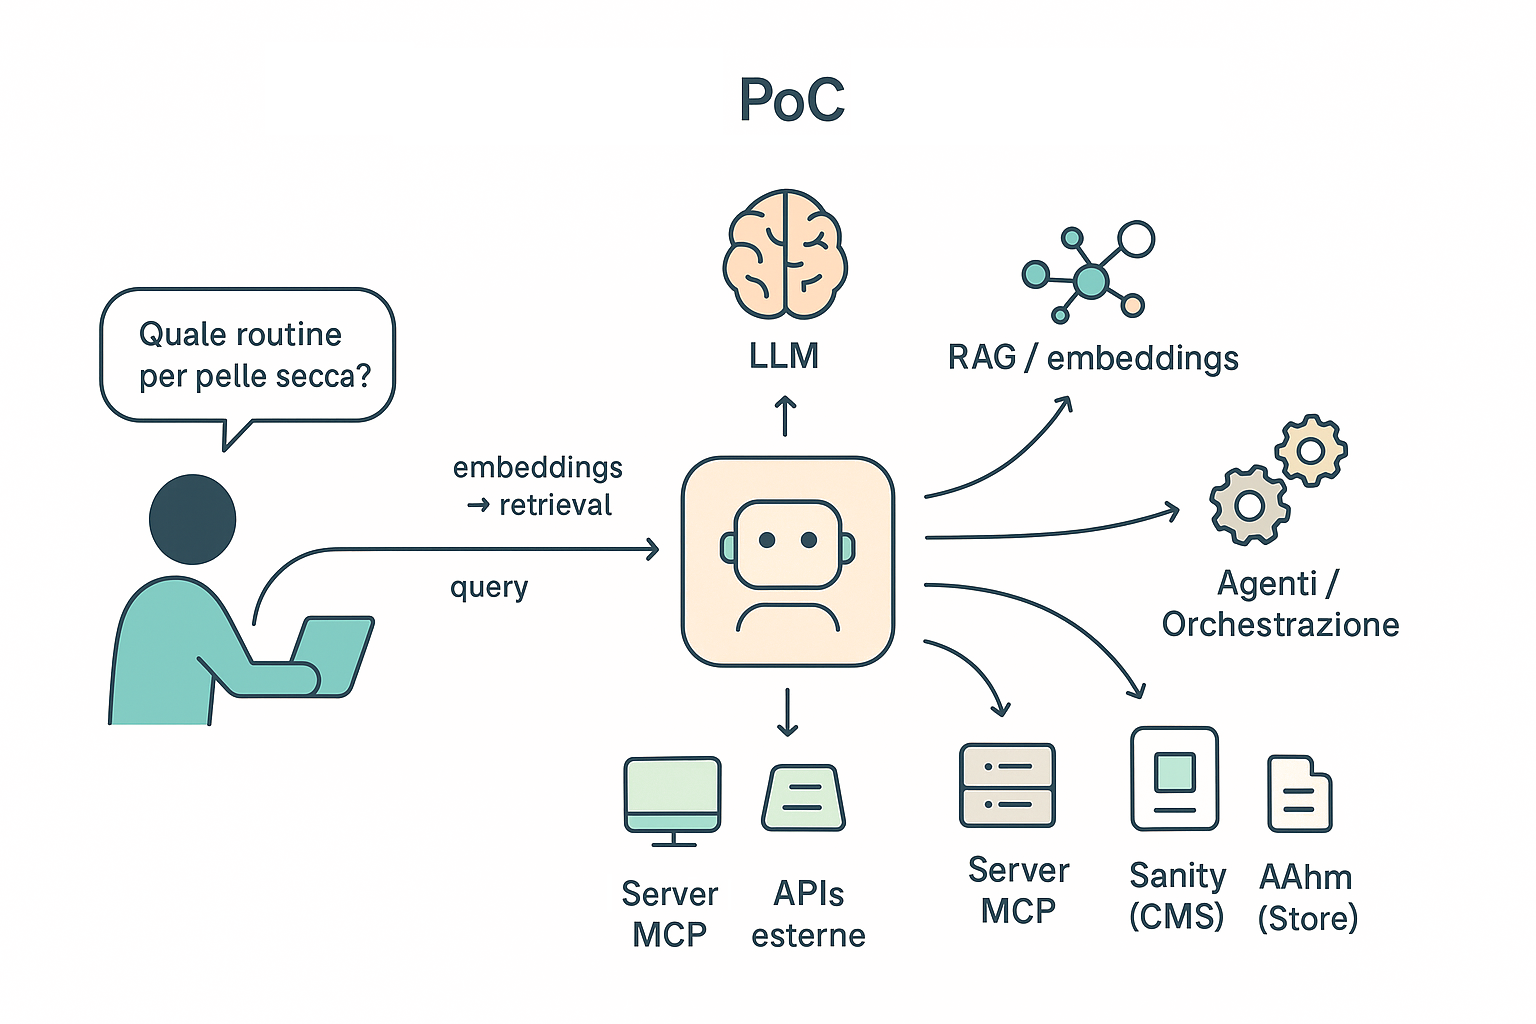
\includegraphics[width=0.8\textwidth]{stage/progetto}
    \caption{Composizione del \emph{Proof of Concept}.}
    \label{fig:progetto}
  \end{figure}
%%%
Dal punto di vista applicativo, il progetto è stato concepito per affrontare un problema concreto del dominio della \emph{skin-care}: la complessità informativa 
che spesso ostacola l’utente nella navigazione di un catalogo ampio e specializzato. 
Il fenomeno di \emph{overwhelming}, ossia il sovraccarico cognitivo derivante dall’eccesso di informazioni, rappresenta una delle principali sfide per gli \emph{e-commerce} del settore. 
Il sistema proposto mira a ridurre tale complessità, fungendo da mediatore intelligente capace di comprendere le richieste dell’utente, fornire spiegazioni, suggerire routine personalizzate, 
verificare la compatibilità tra prodotti e individuare soluzioni mirate alle esigenze espresse. 
In questo modo, il progetto contribuisce anche al miglioramento dell’esperienza utente (\emph{User Experience}, \emph{UX}).
%%%
\begin{figure}[H]
    \centering
    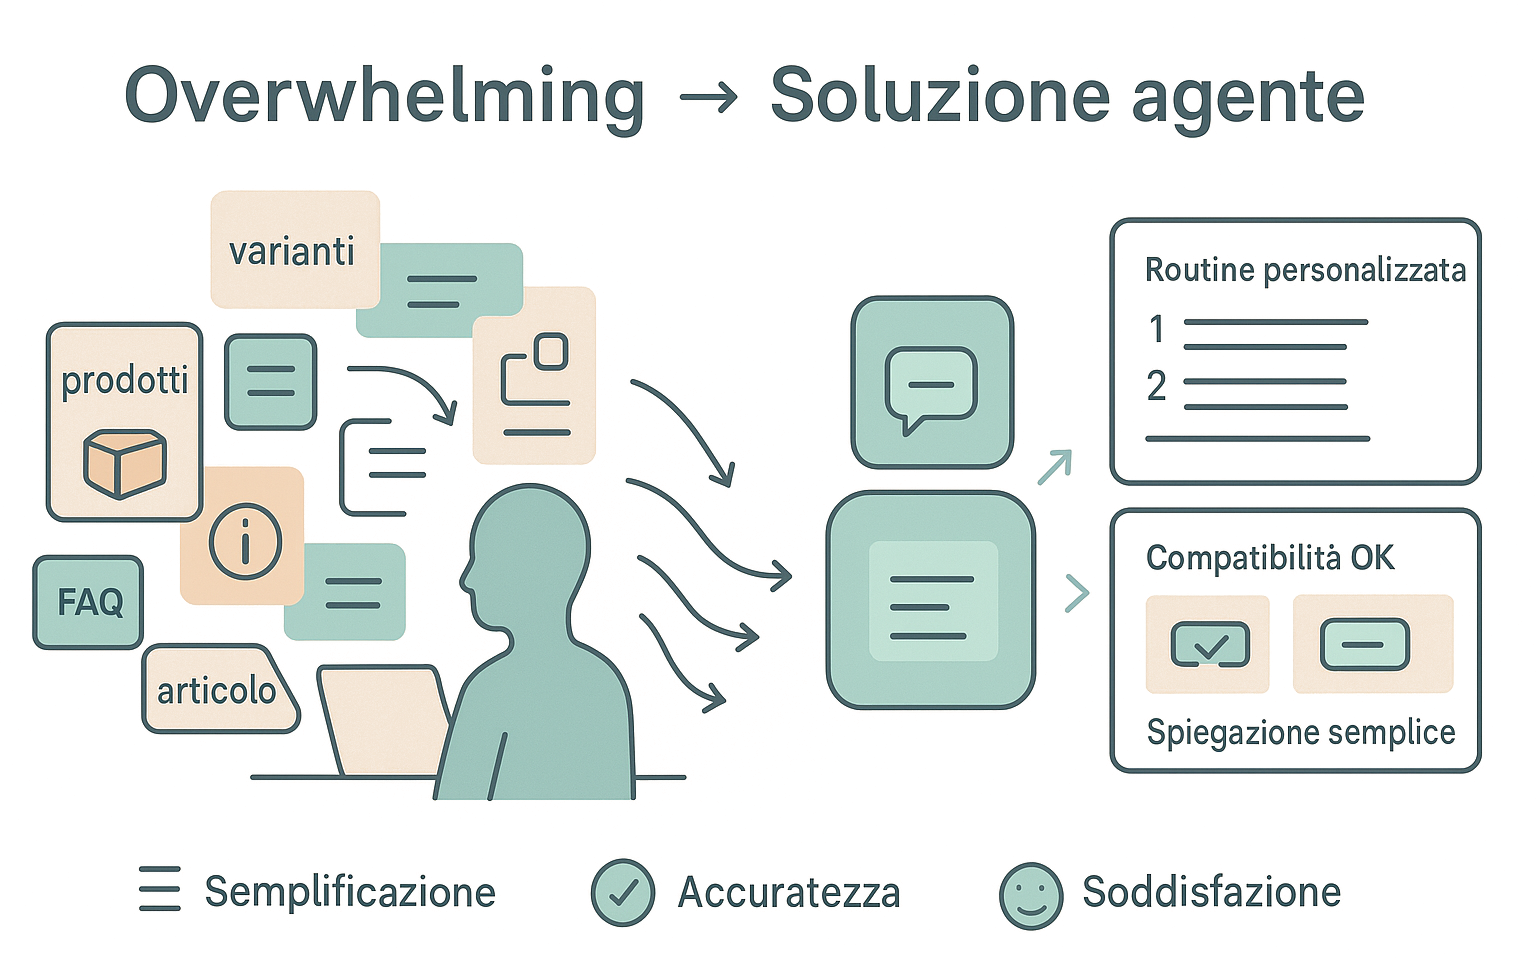
\includegraphics[width=0.8\textwidth]{stage/overwhelming}
    \caption{Il fenomeno di \emph{overwhelming} a confronto con un mediatore intelligente.}
    \label{fig:overwhelming}
  \end{figure}
%%%
Lo \emph{stage}, per sua natura esplorativa, non è stato rigidamente vincolato a un insieme fisso di tecnologie o metodologie, ma ha lasciato spazio alla 
sperimentazione e all’adattamento progressivo. 
I vincoli principali hanno riguardato l’utilizzo di \emph{Shopify} per la gestione del canale \emph{e-commerce} e di \emph{Sanity} 
come \emph{CMS}, in quanto piattaforme già adottate dall’azienda ospitante e quindi imprescindibili per garantire compatibilità e continuità con l’infrastruttura esistente.

Dal punto di vista operativo e temporale, il progetto è stato suddiviso in più fasi: una prima fase di studio delle tecnologie e di definizione dei requisiti, 
una seconda fase di progettazione architetturale e sperimentazione su un \emph{playground} (ambiente di test interattivo per sperimentare codice o configurazioni in modo sicuro), e infine una fase di sviluppo del \emph{PoC} vero e proprio, con attività di test e validazione. 
Il lavoro si è svolto in stretto coordinamento con il tutor aziendale, che ha svolto un ruolo chiave di guida e confronto tecnico-strategico, garantendo la coerenza tra 
le scelte progettuali e la visione di innovazione perseguita dall’azienda. 
In particolare, il tutor ha contribuito alla definizione del perimetro di sperimentazione e 
ha condotto in parallelo analisi comparative di tecnologie affini a quelle testate, al fine di valutare concretamente i possibili \emph{trade-off} (compromesso tra due o più aspetti in conflitto, dove migliorare uno comporta peggiorare l’altro) e ottimizzare i tempi di sviluppo.
%%%
\begin{figure}[H]
    \centering
    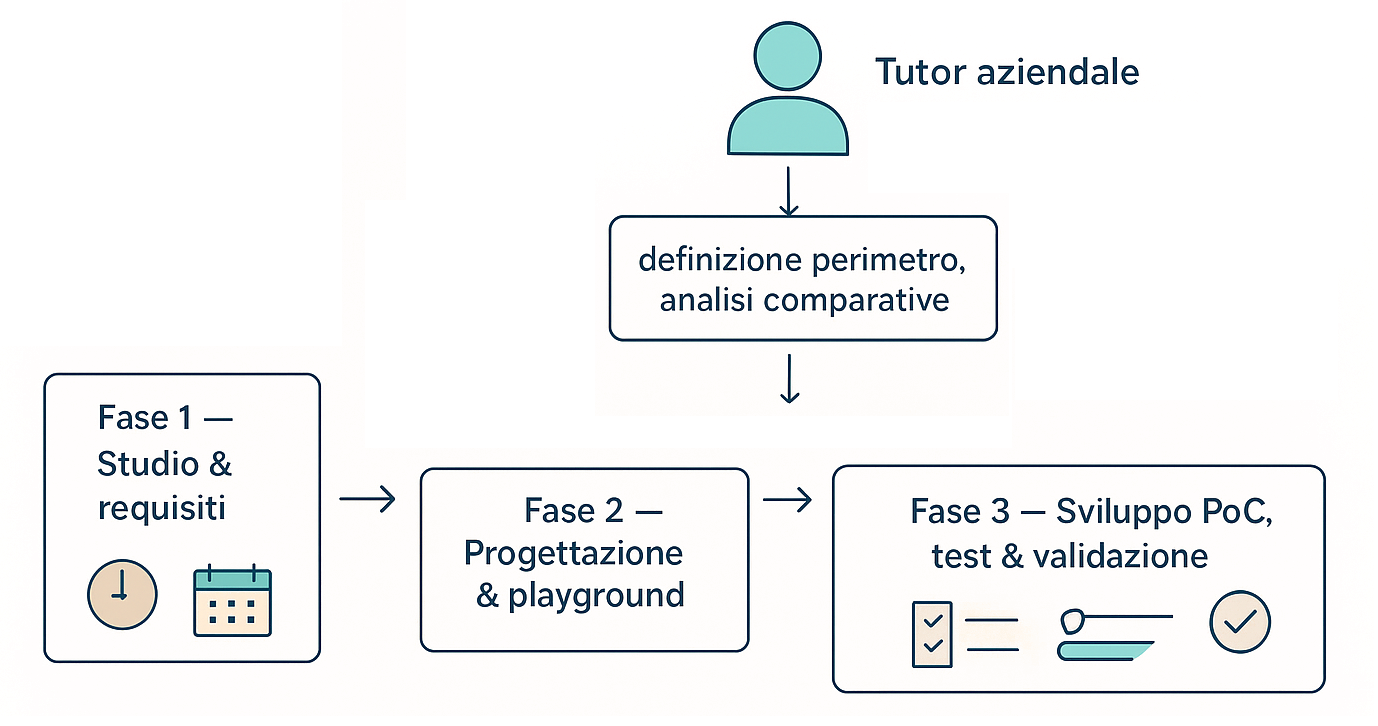
\includegraphics[width=0.8\textwidth]{stage/fasi_progetto}
    \caption{La suddivisione in fasi del progetto con sviluppo parallelo da parte del tutor aziendale.}
    \label{fig:fasi_progetto}
  \end{figure}
%%%
L’approccio adottato è stato volutamente “morbido” riguardo agli obiettivi, permettendo di ampliare progressivamente il perimetro del progetto in base ai risultati ottenuti. 
Tale flessibilità ha favorito una gestione dinamica dello \emph{stage}, nella quale obiettivi iniziali più cauti sono stati progressivamente integrati con traguardi più ambiziosi, 
mantenendo però un’attenzione costante alla fattibilità e all’efficienza economica. 
Il vincolo principale, oltre alla compatibilità tecnologica, è stato quello di privilegiare soluzioni semplici, modulabili e pronte alla distribuzione, evitando la tendenza a “reinventare la ruota” 
e promuovendo invece un approccio pragmatico, centrato sull’utente e orientato al valore concreto per l’azienda.
%%%
\begin{figure}[H]
    \centering
    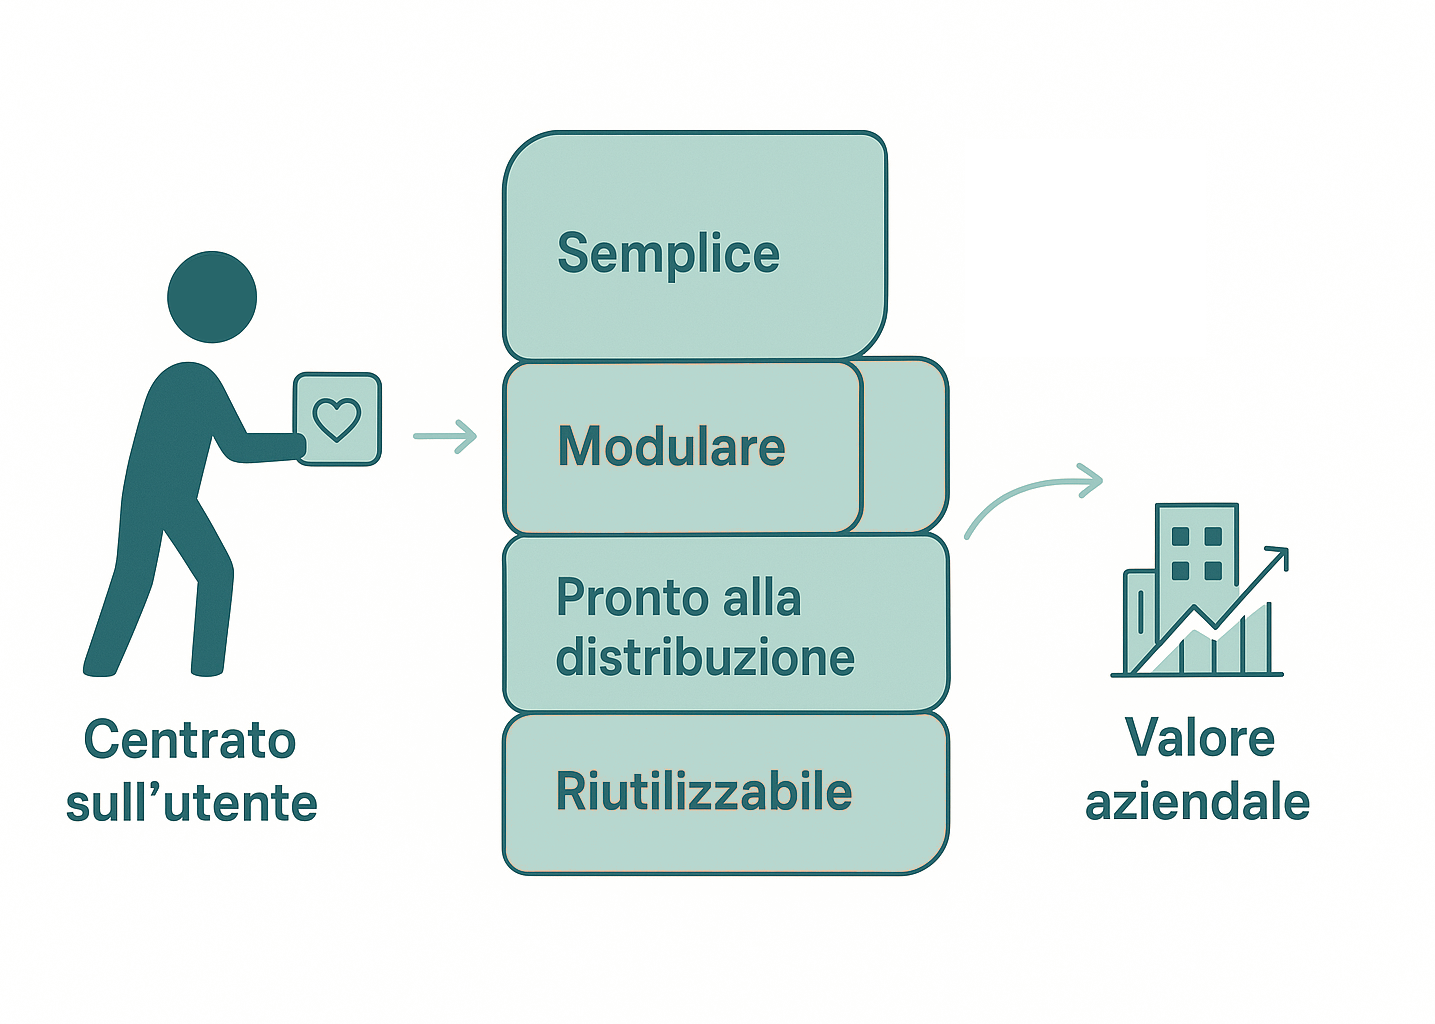
\includegraphics[width=0.8\textwidth]{stage/vincolo_architetturale}
    \caption{Approccio di lavoro flessibile e pragmatico.}
    \label{fig:vincolo_architetturale}
\end{figure}
%%%
%Questo progetto di \emph{stage} riflette pienamente la strategia di innovazione dell’organizzazione ospitante, che vede negli \emph{stage} 
%e nei progetti sperimentali uno strumento essenziale per esplorare nuove tecnologie, testarne le applicazioni in contesti reali e formare competenze interne. 
%L’azienda, infatti, adotta una visione di innovazione incrementale, basata su iterazioni successive di apprendimento e validazione, piuttosto che su approcci 
%radicali e ad alto rischio. In questa prospettiva, lo \emph{stage} non rappresenta un episodio isolato, ma una parte di un processo più ampio di evoluzione tecnologica, 
%volto a migliorare la competitività del brand attraverso soluzioni digitali sempre più personalizzate e intelligenti.

Al termine dello \emph{stage}, è stata prevista la consegna di tutta la documentazione tecnica e dei risultati del \emph{PoC}, in modo da permettere all’azienda di proseguire in 
autonomia lo sviluppo e valutare la possibilità di una futura industrializzazione del prototipo.








% attività di supporto previste prima, durante e dopo il periodo di tirocinio




%Sezione in cui verrà illustrato il progetto di stage ricevuto, esplicitando le problematiche applicative che l'organizzazione intende affrontare con il tirocinio, 
%gli obiettivi specifici prefissati e i vincoli operativi e temporali associati. Verrà inoltre evidenziato il rapporto tra la proposta di stage e la strategia più ampia dell'ente ospitante 
%in materia di innovazione (con riferimento al ruolo e alla posizione assunta dal tutor aziendale emerse nel primo incontro) 
%nonché le attività di supporto previste prima, durante e dopo il periodo di tirocinio.
%Qui concluderò la trattazione del punto 2 (perché) riportato nel file Struttura relazione finale.pdf.